% Provenance (never printed): see sources/outline_sources.md (Year 3:
% atmospheric dynamics: vorticity and potential vorticity, Rossby waves,
% baroclinic instability, the general circulation and the Hadley cell).
% Brief: sources/book5/BRIEFS.md, ch. 20. Curves from
% figdata/bachelor-3/rossby_waves.py, eady.py and held_hou.py. Exercise and
% problem values in the Book 5 scratch calculator calc/ch20.py. The waves,
% shears and parcels of the exercises and the problem are invented.
\chapter{Dynamique atmosphérique}\label{ch:b3:atmospheric-dynamics}

Sur une carte hivernale de la haute troposphère, le courant-jet ne ceinture pas
le pôle en un anneau régulier. Il serpente, en quelques grandes ondes autour de
l'hémisphère, avec des creux descendant vers les subtropiques et des crêtes vers le
pôle, et en surface naissent des dépressions qui croissent pendant quelques jours et meurent
sous elles. Les ondes dérivent lentement, parfois à contre-courant du vent qui
les porte. Leur nombre, leur vitesse et la croissance des tempêtes situées dessous
découlent d'une même grandeur conservée, la vorticité de l'air vue depuis
l'espace, et de l'énergie emmagasinée dans le contraste thermique entre les
tropiques et les pôles.

\begin{recall}
La vorticité et la circulation sont dans les volumes de physique. Les ondes de Rossby de la
haute troposphère, les creux et les crêtes, le cyclone extratropical et le
principe de la prévision numérique du temps sont décrits dans le
volume de deuxième année, dans son chapitre sur les systèmes météorologiques. Les cellules de Hadley, de Ferrel et
polaires, les courants-jets, les vents d'ouest et le vent de moment cinétique d'un anneau
d'air sont dans le volume de première année, dans son chapitre sur la circulation générale de
l'atmosphère, et le transport de chaleur vers les pôles, dans son chapitre sur
le rayonnement et le transport de chaleur. Le paramètre de Coriolis $f$, le plan $\beta$,
le rayon de Rossby et le \omterm{thm:b3:gfd-foundations:thermal-wind}{vent thermique} figurent au
chapitre~\ref{ch:b3:gfd-foundations}.
\end{recall}

\section{Vorticité}\label{sec:b3:atmospheric-dynamics:vorticity}

La vorticité d'un fluide, le rotationnel de sa vitesse, vaut deux fois sa
vitesse angulaire locale. Pour l'atmosphère à grande échelle, seule sa composante
verticale compte, et la rotation de la Terre y contribue.

\begin{definition}[Vorticité relative, planétaire et absolue]\label{def:b3:atmospheric-dynamics:vorticity-kinds}
Pour une vitesse horizontale $(u, v)$, la \emph{vorticité
relative}\index{vorticité relative} est la composante verticale du rotationnel
de la vitesse relative au sol, $\zeta = \partial v/\partial x -
\partial u/\partial y$, positive pour une rotation antihoraire vue d'en haut.
La \emph{vorticité planétaire}\index{vorticité planétaire} est la composante verticale
de la vorticité de la rotation terrestre, $2\Omega\sin\varphi =
f$. La \emph{vorticité absolue}\index{vorticité absolue} est leur somme,
$\zeta + f$.
\end{definition}

Dans l'hémisphère Nord, une dépression, où l'air tourne dans le sens antihoraire,
a $\zeta > 0$ et est dite cyclonique~; un anticyclone a $\zeta < 0$. Un
vent de \qty{15}{m/s} tournant sur un cercle de \qty{1000}{km} a $\zeta =
2V/R = \qty{3e-5}{s^{-1}}$ en rotation solide, soit un tiers de $f$ à \ang{45}~:
la partie planétaire est en général la plus grande.

\begin{theorem}[Équation de la vorticité barotrope]\label{thm:b3:atmospheric-dynamics:bve}
Dans un écoulement non visqueux, bidimensionnel et sans divergence horizontale sur un
plan $\beta$, la \omterm{def:b3:atmospheric-dynamics:vorticity-kinds}{vorticité absolue} de chaque particule est conservée~:
\[
\frac{\mathrm D(\zeta + f)}{\mathrm Dt} = 0 ,
\qquad\text{soit}\qquad
\frac{\partial\zeta}{\partial t} + u\frac{\partial\zeta}{\partial x} + v\frac{\partial\zeta}{\partial y} + \beta v = 0 .
\]
C'est l'\emph{équation de la vorticité barotrope}\index{equation@équation de la vorticité barotrope}.
\end{theorem}

\begin{proof}
Les équations horizontales du mouvement sont $\mathrm Du/\mathrm Dt - fv =
-(1/\rho_0)\partial p/\partial x$ et $\mathrm Dv/\mathrm Dt + fu =
-(1/\rho_0)\partial p/\partial y$. On dérive la seconde par rapport à
$x$, la première par rapport à $y$, et on soustrait~: la pression disparaît.
Avec $\delta = \partial u/\partial x + \partial v/\partial y$, les termes
advectifs donnent $\partial_x(u\,\partial_xv + v\,\partial_yv) -
\partial_y(u\,\partial_xu + v\,\partial_yu) = u\,\partial_x\zeta +
v\,\partial_y\zeta + \zeta\delta$, et les termes de Coriolis $f\delta + \beta
v$. D'où $\mathrm D\zeta/\mathrm Dt + \beta v = -(\zeta + f)\,\delta$. Pour
$\delta = 0$, et puisque $\mathrm Df/\mathrm Dt = \beta v$, $\mathrm D(\zeta +
f)/\mathrm Dt = 0$.
\end{proof}

La démonstration donne aussi la loi générale, $\mathrm D(\zeta + f)/\mathrm Dt =
-(\zeta + f)\delta$~: la convergence accélère la rotation d'une colonne, la divergence
la freine, comme une patineuse qui rapproche les bras du corps ou les écarte. Dans une couche dont
l'épaisseur varie, la convergence est liée à l'étirement de la colonne, et
la grandeur conservée devient un rapport.

\begin{definition}[Vorticité potentielle]\label{def:b3:atmospheric-dynamics:pv}
La \emph{vorticité potentielle}\index{vorticité potentielle} d'une colonne d'une
couche homogène d'épaisseur $h$ est $q = (\zeta + f)/h$. Dans un fluide continûment
stratifié, la vorticité potentielle d'Ertel est $q = (\vec\omega_a\cdot
\nabla\theta)/\rho$, avec $\vec\omega_a$ le vecteur de \omterm{def:b3:atmospheric-dynamics:vorticity-kinds}{vorticité absolue} et
$\theta$ la température potentielle.
\end{definition}

\begin{theorem}[Conservation de la vorticité potentielle]\label{thm:b3:atmospheric-dynamics:pv}
Dans une couche homogène, hydrostatique et non visqueuse, d'épaisseur variable $h$ dont
la vitesse horizontale ne varie pas avec la hauteur, $\mathrm Dq/\mathrm Dt = 0$
pour $q = (\zeta + f)/h$.
\end{theorem}

\begin{proof}
D'après la démonstration ci-dessus, $\mathrm D(\zeta + f)/\mathrm Dt = -(\zeta + f)\delta$.
La conservation de la masse dans une colonne de masse volumique uniforme donne $\mathrm Dh/\mathrm
Dt = -h\delta$. Puis $\mathrm Dq/\mathrm Dt = (1/h)\,\mathrm D(\zeta +
f)/\mathrm Dt - ((\zeta + f)/h^2)\,\mathrm Dh/\mathrm Dt = -(\zeta +
f)\delta/h + (\zeta + f)\delta/h = 0$.
\end{proof}

La forme d'Ertel se conserve de la même façon lors d'un écoulement adiabatique et sans
frottement d'un fluide stratifié, la distance entre deux surfaces à
$\theta$ constant jouant le rôle de $h$. Une colonne d'air franchissant une chaîne de
montagnes est comprimée lors de la montée~: sa \omterm{def:b3:atmospheric-dynamics:vorticity-kinds}{vorticité absolue} diminue, elle tourne
de façon anticyclonique au-dessus de la crête, puis elle s'étire et tourne
cycloniquement sous le vent. La conservation de
la \omterm{def:b3:atmospheric-dynamics:vorticity-kinds}{vorticité absolue} ou potentielle est le mécanisme de rappel des ondes
de la section suivante, comme le montre la figure ci-dessous.

\begin{omfigure}
\begin{tikzpicture}[>=stealth, font=\small, declare function={w(\x)=0.9*sin(\x r);}]
\draw[black!40, dashed] (0,0) -- (12.6,0) node[right, font=\scriptsize] {latitude $\varphi_0$};
\draw[thick, omDef, domain=0:12.566, samples=120] plot (\x, {w(\x)});
\foreach \x in {0.785, 2.356, 3.927, 5.498, 7.069, 8.639, 10.21, 11.78}
  \fill (\x, {w(\x)}) circle (0.06);
% crests: clockwise (anticyclonic), troughs: anticlockwise (cyclonic)
\foreach \x in {1.571, 7.854} {
  \draw[->, omThm, thick] (\x+0.45,{w(\x)+0.05}) arc (0:-300:0.45);
  \node[font=\scriptsize, omThm] at (\x,{w(\x)+0.75}) {$\zeta < 0$};}
\foreach \x in {4.712, 10.996} {
  \draw[->, omMeth, thick] (\x+0.45,{w(\x)-0.05}) arc (0:300:0.45);
  \node[font=\scriptsize, omMeth] at (\x,{w(\x)-0.75}) {$\zeta > 0$};}
\foreach \x in {3.1416, 9.4248} \draw[->, very thick] (\x,0.45) -- (\x,-0.45);
\foreach \x in {6.2832} \draw[->, very thick] (\x,-0.45) -- (\x,0.45);
\draw[->, thick] (8.4,-2.25) -- (6.4,-2.25) node[left, font=\scriptsize] {le motif se déplace vers l'ouest};
\draw[->] (0,-2.25) -- (1.4,-2.25) node[right, font=\scriptsize] {est};
\draw[->] (0,-2.25) -- (0,-1.65) node[above, font=\scriptsize] {nord};
\end{tikzpicture}

\par\smallskip{\small Déplacement d'une onde de Rossby (schéma, hémisphère
Nord). Une chaîne de parcelles au repos à la latitude $\varphi_0$ est
déplacée en onde. En conservant $\zeta + f$, les parcelles déplacées vers le nord, où
$f$ est plus grande, acquièrent une \omterm{def:b3:atmospheric-dynamics:vorticity-kinds}{vorticité relative} anticyclonique~; celles déplacées vers le sud,
cycloniques. Entre une crête et le creux situé à son est, l'écoulement induit
est dirigé vers le sud, entre un creux et la crête située à son est vers le nord (flèches
noires)~: le déplacement croît à l'ouest de chaque crête et l'ensemble du motif
se décale vers l'ouest.}\label{fig:b3:atmospheric-dynamics:restoring}
\end{omfigure}

\section{Ondes de Rossby}\label{sec:b3:atmospheric-dynamics:rossby}

Le volume de deuxième année décrivait les ondes de Rossby de la haute troposphère. On
les explique par l'\omterm{thm:b3:atmospheric-dynamics:bve}{équation de la vorticité barotrope}. Écrivons l'écoulement comme un
vent d'ouest uniforme $U$ plus une petite perturbation de fonction de courant $\psi'$, de sorte que
$u' = -\partial\psi'/\partial y$, $v' = \partial\psi'/\partial x$ et $\zeta'
= \nabla^2\psi'$.

\begin{theorem}[Dispersion des ondes de Rossby]\label{thm:b3:atmospheric-dynamics:rossby}
De petites perturbations $\psi' \propto \mathrm e^{\mathrm i(kx + ly - \omega t)}$
d'un vent d'ouest uniforme $U$ sur un plan $\beta$ obéissent à la
\emph{relation de dispersion des ondes de Rossby}\index{relation de dispersion des ondes de Rossby}
\[
\omega = Uk - \frac{\beta k}{k^2 + l^2} .
\]
Leur vitesse de phase vers l'est est $c = \omega/k = U - \beta/K^2$, avec $K^2 =
k^2 + l^2$, et leur vitesse de groupe vers l'est $c_g = \partial\omega/\partial
k = U + \beta(k^2 - l^2)/K^4$.
\end{theorem}

\begin{proof}
Linéarisée autour de $U$, l'\omterm{thm:b3:atmospheric-dynamics:bve}{équation de la vorticité barotrope} s'écrit
$(\partial_t + U\partial_x)\nabla^2\psi' + \beta\,\partial_x\psi' = 0$, les
produits de petites quantités étant négligés et $\zeta$ de l'écoulement de base
étant nul. Pour l'onde plane, $\partial_t \to -\mathrm i\omega$,
$\partial_x \to \mathrm ik$ et $\nabla^2 \to -K^2$~: $(-\mathrm i\omega +
\mathrm iUk)(-K^2) + \mathrm i\beta k = 0$, soit $(\omega - Uk)K^2 =
-\beta k$. En dérivant $\omega$ par rapport à $k$, on obtient $c_g = U -
\beta/K^2 + 2\beta k^2/K^4$, ce qui est la forme annoncée.
\end{proof}

\begin{omfigure}
\begin{tikzpicture}
\begin{groupplot}[group style={group size=2 by 1, horizontal sep=1.7cm},
  width=0.48\linewidth, height=0.46\linewidth, tick label style={font=\scriptsize},
  label style={font=\small}, legend style={font=\scriptsize, draw=none, fill=none}]
\nextgroupplot[xlabel={nombre d'onde zonal $n$}, ylabel={vitesse (\unit{m/s})},
  xmin=1, xmax=12, ymin=-40, ymax=60, legend pos=north east, legend cell align=left,
  title={\small \ang{45} N}]
% computed in figdata/bachelor-3/rossby_waves.py
\addplot[omThm, thick] table[x=n, y=c15] {figdata/out/bachelor-3-rossby_waves-disp.dat};
\addlegendentry{$c$, $U = 15$}
\addplot[omThm, thick, densely dashed] table[x=n, y=cg15] {figdata/out/bachelor-3-rossby_waves-disp.dat};
\addlegendentry{$c_g$, $U = 15$}
\addplot[omDef, thick] table[x=n, y=c0] {figdata/out/bachelor-3-rossby_waves-disp.dat};
\addlegendentry{$c$, $U = 0$}
\addplot[omDef, thick, densely dashed] table[x=n, y=cg0] {figdata/out/bachelor-3-rossby_waves-disp.dat};
\addlegendentry{$c_g$, $U = 0$}
\addplot[black!50, thin, domain=1:12, samples=2, forget plot] {0};
\nextgroupplot[xlabel={latitude (\unit{\degree} N)}, ylabel={nombre d'onde stationnaire $n_s$},
  xmin=20, xmax=75, ymin=0, ymax=9, legend pos=north east, legend cell align=left]
\addplot[omMeth, thick] table[x=lat, y=n10] {figdata/out/bachelor-3-rossby_waves-stat.dat};
\addplot[omDef, thick] table[x=lat, y=n15] {figdata/out/bachelor-3-rossby_waves-stat.dat};
\addplot[omThm, thick] table[x=lat, y=n20] {figdata/out/bachelor-3-rossby_waves-stat.dat};
\addplot[black, only marks, mark=*, mark size=1.1pt] table[x=lat, y=ns] {figdata/out/bachelor-3-rossby_waves-statobs.dat};
\legend{\qty{10}{m/s}, \qty{15}{m/s}, \qty{20}{m/s}, janvier \qty{300}{hPa}}
\end{groupplot}
\end{tikzpicture}

\par\smallskip{\small À gauche, la vitesse de phase vers l'est $c$ (trait plein) et la
vitesse de groupe $c_g$ (tirets) des ondes de Rossby avec $l = 0$ à \ang{45} N, en fonction
le nombre d'ondes le long du cercle de latitude, sans vent moyen (bleu)
et dans un vent d'ouest de \qty{15}{m/s} (rouge)~: les ondes longues se déplacent vers l'ouest, les courtes
sont entraînées vers l'est, et $c_g > c$. À droite, le nombre d'onde stationnaire pour
des vents d'ouest uniformes de 10, 15 et \qty{20}{m/s}, et pour le vent zonal moyen de janvier
à \qty{300}{hPa} à chaque latitude (points, NCEP--NCAR
Reanalysis~1, 1991--2020).}\label{fig:b3:atmospheric-dynamics:rossby}
\end{omfigure}
% ledger: data:b5-ncep-uwnd, geod5:grs80-defining, earth:Rmean

Par rapport à l'air, les ondes se déplacent toujours vers l'ouest, d'autant plus
vite qu'elles sont longues. Un vent d'ouest entraîne vers l'est les ondes courtes~; les longues
qu'il ne peut pas entraîner, et elles dérivent vers l'ouest, à contre-courant. Entre les deux,
une longueur d'onde reste immobile.

\begin{proposition}[Ondes de Rossby stationnaires]\label{prop:b3:atmospheric-dynamics:stationary}
Dans un vent d'ouest $U > 0$, une onde sans structure méridienne ($l = 0$) est
stationnaire lorsque sa longueur d'onde est égale à la \emph{longueur d'onde stationnaire
de Rossby}\index{longueur d'onde stationnaire de Rossby} $\lambda_s =
2\pi\sqrt{U/\beta}$. Sur le cercle de latitude $\varphi$, cela correspond à un
nombre entier d'ondes voisin de $n_s = \sqrt{2\Omega a\cos^3\varphi/U}$.
\end{proposition}

\begin{proof}
$c = 0$ lorsque $k^2 = \beta/U$, donc $\lambda_s = 2\pi/k = 2\pi\sqrt{U/\beta}$.
Le cercle a pour longueur $2\pi a\cos\varphi$, donc $n_s = a\cos\varphi\,k =
a\cos\varphi\sqrt{2\Omega\cos\varphi/(aU)} = \sqrt{2\Omega a\cos^3\varphi/U}$.
\end{proof}

À \ang{45} N, dans un vent d'ouest de \qty{15}{m/s}, avec $\beta =
\qty{1.62e-11}{m^{-1}.s^{-1}}$, on a $\lambda_s = \qty{6050}{km}$ et $n_s =
4.7$~: quatre ou cinq ondes font le tour de l'hémisphère. Avec le vent zonal moyen
de janvier à \qty{300}{hPa}, d'environ \qty{21}{m/s} à \ang{45} N, $n_s$
vaut environ quatre de \ang{35} à \ang{55} N, et diminue vers le pôle. La vitesse
de groupe d'une onde avec $l = 0$ dépasse sa vitesse de phase de $2\beta/k^2$~:
l'énergie court en avant de l'onde, de sorte qu'une perturbation déclenchée en
un lieu construit de nouveaux creux et crêtes en aval, quelques jours plus tard
et des milliers de kilomètres plus à l'est, tandis que la configuration elle-même
bouge à peine. Les chaînes de montagnes et les contrastes de température entre
continents et océans forcent des ondes stationnaires de ce type, par l'étirement
et la compression de la \omterm{def:b3:atmospheric-dynamics:pv}{vorticité potentielle}.
% ledger: geod5:grs80-defining, earth:Rmean, data:b5-ncep-uwnd (values in figdata/bachelor-3/rossby_waves.py)


\section{Instabilité barocline}\label{sec:b3:atmospheric-dynamics:baroclinic}

Les ondes de la section précédente sont neutres~: elles ne croissent ni ne décroissent.
Les tempêtes des latitudes moyennes croissent, et puisent leur énergie dans le
contraste de température qu'exprime le \omterm{thm:b3:gfd-foundations:thermal-wind}{vent thermique}.

\begin{definition}[Énergie potentielle disponible]\label{def:b3:atmospheric-dynamics:ape}
L'\emph{énergie potentielle disponible}\index{energie@énergie potentielle disponible} d'un
fluide stratifié est la différence entre son énergie potentielle totale
(gravitationnelle et interne) et la plus petite énergie potentielle totale
qu'il puisse atteindre par un réarrangement adiabatique de sa masse, c'est-à-dire
l'état dans lequel les surfaces de température potentielle constante, ou de
densité potentielle constante, sont horizontales.
\end{definition}

Un fluide aux isentropes horizontales n'en possède aucune, quelle que soit
l'énergie potentielle qu'il renferme~; un fluide dont les isentropes sont
inclinées, chaudes et légères d'un côté, froides et denses de l'autre, peut
en libérer une partie en les laissant s'affaisser. L'échange de deux particules
le montre. Prenons une particule chaude basse du côté de l'équateur et une
particule froide haute du côté du pôle, toutes deux sur la même isentrope dans
une atmosphère stable dont les isentropes remontent vers le pôle. Les échanger
le long de l'isentrope ne change rien. Les échanger le long d'un chemin moins
pentu que l'isentrope fait monter la particule chaude vers le pôle et vers le haut,
dans un air plus froid qu'elle, et faire descendre la particule froide vers
l'équateur, dans un air plus chaud~: la chaude monte, la froide descend, le centre
de masse s'abaisse, et de l'énergie cinétique est libérée. Les trajets situés
dans ce coin compris entre l'horizontale et les isentropes libèrent de l'énergie~; les \omterm{def:b3:atmospheric-dynamics:eddy}{tourbillons} des latitudes moyennes sont de tels échanges, qui transportent la chaleur vers le pôle et vers le haut.

\begin{definition}[Instabilité barocline]\label{def:b3:atmospheric-dynamics:baroclinic-instability}
L'\emph{instabilité barocline}\index{instabilité barocline} est l'instabilité d'un
écoulement en rotation et stratifié, en équilibre de \omterm{thm:b3:gfd-foundations:thermal-wind}{vent thermique}, par laquelle
les perturbations croissent en convertissant l'\omterm{def:b3:atmospheric-dynamics:ape}{énergie potentielle disponible} des
isentropes inclinées en leur propre énergie cinétique.
\end{definition}

\begin{definition}[Modèle d'Eady]\label{def:b3:atmospheric-dynamics:eady}
Le \emph{modèle d'Eady}\index{modèle d'Eady} est un fluide de Boussinesq sur un
plan $f$ compris entre deux surfaces horizontales rigides en $z = 0$ et $z = H$, avec
une \omterm{def:b3:gfd-foundations:buoyancy}{fréquence de flottabilité} uniforme $N$ et un vent d'ouest qui croît linéairement
avec la hauteur, $U = \Lambda z$, en équilibre de \omterm{thm:b3:gfd-foundations:thermal-wind}{vent thermique} avec une décroissance
uniforme de la température vers le pôle~; ses perturbations obéissent aux
équations quasi-géostrophiques.
\end{definition}

\begin{theorem}[Taux de croissance d'Eady]\label{thm:b3:atmospheric-dynamics:eady}
Dans le \omterm{def:b3:atmospheric-dynamics:eady}{modèle d'Eady}, les perturbations $\propto \mathrm e^{\mathrm ik(x - ct)}$
avec $\mu = kL_d$, $L_d = NH/f$, croissent exponentiellement lorsque $\mu < \mu_c =
2.40$, au taux
\[
\sigma = \frac{f\Lambda}{N}\left[\left(\coth\frac{\mu}{2} - \frac{\mu}{2}\right)\left(\frac{\mu}{2} - \tanh\frac{\mu}{2}\right)\right]^{1/2} .
\]
La perturbation qui croît le plus vite a $\mu = 1.61$, la longueur d'onde $2\pi L_d/1.61
\approx 3.9\,L_d$, et croît à $\sigma_{\max} = 0.31\,f\Lambda/N$.
\end{theorem}
\admitted

Le taux de croissance ne dépend que du cisaillement et de la stratification, à
travers $f\Lambda/N$, et la taille privilégiée seulement du rayon de Rossby. Pour la
moyenne de janvier à \ang{45} N, le vent augmente de \qty{17.2}{m/s} entre
\qty{850}{hPa} et \qty{250}{hPa}, à environ \qty{8.9}{km} d'écart dans
l'atmosphère standard, soit un cisaillement de \qty{1.9e-3}{s^{-1}}~; avec la
stratification moyenne de la troposphère $N = \qty{0.0113}{s^{-1}}$ et $H = \qty{11}{km}$, on a $L_d =
\qty{1210}{km}$, la perturbation la plus rapide a une longueur d'onde de \qty{4700}{km}
et croît d'un facteur $e$ en \num{2.1}~jours. Les perturbations plus courtes que
\qty{3200}{km} ne croissent pas du tout. Ce sont là la taille et le temps de
croissance des dépressions sur une carte météorologique.
% ledger: data:b5-ncep-uwnd, nasa:grc-atmos (values in figdata/bachelor-3/eady.py)

\begin{omfigure}
\begin{minipage}[c]{0.52\linewidth}\centering
\begin{tikzpicture}
\begin{axis}[width=\linewidth, height=0.85\linewidth, xmin=2, xmax=16, ymin=0, ymax=0.55,
  xlabel={longueur d'onde (\qty{1000}{km})}, ylabel={taux de croissance (\unit{jour^{-1}})},
  tick label style={font=\scriptsize}, label style={font=\small}]
% computed in figdata/bachelor-3/eady.py
\addplot[omThm, thick] table[x expr=\thisrow{lam}/1000, y=sday] {figdata/out/bachelor-3-eady-curve.dat};
\addplot[only marks, mark=*, mark size=1.6pt] coordinates {(4.721,0.4701)};
\node[font=\scriptsize, anchor=west] at (axis cs:5.0,0.49) {\qty{4700}{km}~: $e$-folding \qty{2.1}{d}};
\addplot[black!50, densely dashed] coordinates {(3.160,0) (3.160,0.55)};
\node[font=\scriptsize, anchor=west, black!60] at (axis cs:3.25,0.04) {coupure};
\end{axis}
\end{tikzpicture}
\end{minipage}\hfill
\begin{minipage}[c]{0.44\linewidth}\centering
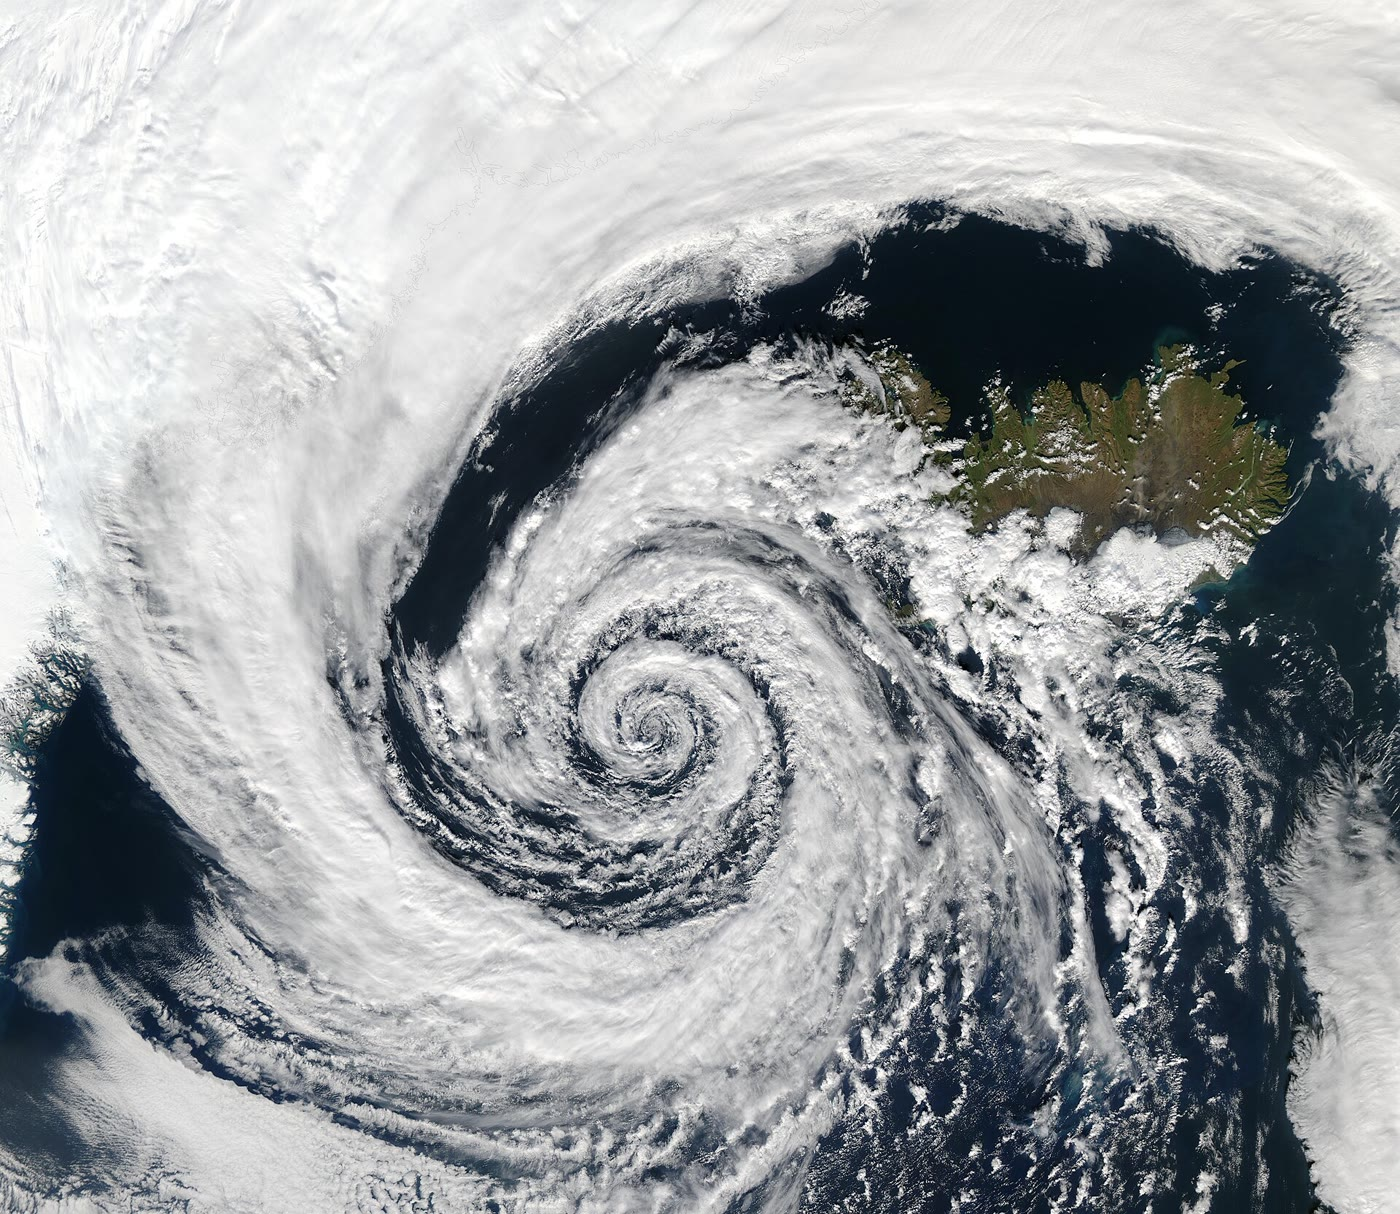
\includegraphics[width=\linewidth]{images/book5/b3-iceland-low.jpg}
\end{minipage}

\par\smallskip{\small À gauche, le taux de croissance d'Eady en fonction de la longueur d'onde pour le
cisaillement zonal moyen de janvier à \ang{45} N (NCEP--NCAR Reanalysis~1,
1991--2020), la stratification moyenne de la troposphère et $H = \qty{11}{km}$~:
pas de croissance en dessous de \qty{3200}{km}, croissance maximale vers \qty{4700}{km}. À droite, une
dépression à son stade mature au large de la côte sud-ouest de l'Islande, le 4
septembre 2003, ses nuages enroulés en spirale anticyclonique autour du
centre bas (NASA/GSFC, MODIS Rapid Response Team,
domaine public).}\label{fig:b3:atmospheric-dynamics:eady}
\end{omfigure}
% ledger: data:b5-ncep-uwnd, nasa:grc-atmos, photo:b3-iceland-low

Le cyclone extratropical du volume de deuxième année est la face de surface d'une
onde \omterm{def:b3:gfd-foundations:baroclinic}{barocline} en croissance~: son secteur chaud transporte l'air chaud vers les pôles et
vers le haut, l'air froid qui le suit glisse vers l'équateur et descend, et le talweg
en altitude s'incline vers l'ouest avec la hauteur, comme l'exige la libération
de l'\omterm{def:b3:atmospheric-dynamics:ape}{énergie potentielle disponible}.

\section{La circulation générale}\label{sec:b3:atmospheric-dynamics:general-circulation}

La circulation générale se décrit en moyennant le long des cercles de latitude,
et ce que la moyenne laisse de côté compte autant que ce qu'elle conserve.

\begin{definition}[Moyenne zonale et tourbillons]\label{def:b3:atmospheric-dynamics:eddy}
La \emph{moyenne zonale}\index{moyenne zonale} d'une grandeur $A$ est sa moyenne
le long d'un cercle de latitude, à altitude ou à pression fixée, $[A] =
(1/2\pi)\int_0^{2\pi} A\,\mathrm d\lambda$. L'écart $A^* = A - [A]$
est sa partie tourbillonnaire~; un \emph{tourbillon}\index{tourbillon (atmosphérique)}
de l'atmosphère est tout écart de l'écoulement à sa moyenne zonale~: ondes
progressives, ondes stationnaires, cyclones et anticyclones.
\end{definition}

La \omterm{def:b3:atmospheric-dynamics:eddy}{moyenne zonale} d'un produit se scinde en deux~: $[vT] = [v][T] + [v^*T^*]$. Le
premier terme est le transport par la circulation méridienne moyenne, les cellules
du volume de première année~; le second est le transport par les \omterm{def:b3:atmospheric-dynamics:eddy}{tourbillons}. Aux
latitudes moyennes, le vent méridien moyen est faible et le terme tourbillonnaire
domine~: l'air qui se dirige vers le pôle est plus chaud que celui qui se dirige
vers l'équateur à la même latitude, comme sur la figure ci-dessous, et $[v^*T^*] > 0$. Les
\omterm{def:b3:atmospheric-dynamics:eddy}{tourbillons} transportent aussi du moment d'ouest, $[u^*v^*]$, depuis les subtropiques vers
les latitudes du courant-jet, ce qui explique que le courant-jet et les vents d'ouest au
sol sont entretenus contre le frottement. La cellule de Ferrel du volume de première
année est la circulation méridienne moyenne que ce transport tourbillonnaire force.

\begin{omfigure}
\begin{tikzpicture}[>=stealth, font=\small, declare function={s(\x)=0.9*sin(\x r); t(\x)=0.9*sin((\x+1.0) r);}]
\draw[thick, black, domain=0:12.566, samples=120] plot (\x, {s(\x)});
\draw[omThm, thick, densely dashed, domain=0:12.566, samples=120] plot (\x, {t(\x)-0.15});
\foreach \x in {0.3, 6.58} {\draw[->, omThm, very thick] (\x,-1.1) -- (\x,1.15)
  node[above, font=\scriptsize] {chaud};}
\foreach \x in {3.45, 9.73} {\draw[->, omDef, very thick] (\x,1.1) -- (\x,-1.15)
  node[below, font=\scriptsize] {froid};}
\node[font=\scriptsize, anchor=west, align=left] at (12.7,{s(12.566)}) {ligne\\de courant};
\node[font=\scriptsize, anchor=west, omThm] at (12.7,{t(12.566)-0.15}) {isotherme};
\draw[->] (-1.6,-1.1) -- (-0.6,-1.1) node[below, font=\scriptsize] {est};
\draw[->] (-1.6,-1.1) -- (-1.6,-0.1) node[above, font=\scriptsize] {nord};
\node[font=\scriptsize] at (6.3,-1.95) {air froid au nord, air chaud au sud};
\end{tikzpicture}

\par\smallskip{\small Une onde \omterm{def:b3:gfd-foundations:baroclinic}{barocline} en croissance, vue en plan (schéma,
hémisphère Nord, écoulement d'ouest). L'isotherme (en pointillés) est en retard sur la
ligne de courant d'un quart de longueur d'onde au plus, si bien que l'air qui se dirige vers le nord (flèches
rouges) est plus chaud que l'air qui se dirige vers le sud à la même latitude (bleues)~:
l'onde transporte la chaleur vers le pôle, $[v^*T^*] >
0$.}\label{fig:b3:atmospheric-dynamics:heatflux}
\end{omfigure}

Dans les tropiques, les \omterm{def:b3:atmospheric-dynamics:eddy}{tourbillons} sont faibles et la circulation moyenne transporte la
chaleur vers le pôle~: la cellule de Hadley. Le volume de première année a établi que
l'air quittant l'équateur au repos et conservant son moment cinétique soufflerait à des centaines de
mètres par seconde à \ang{40}, et laissait en suspens la raison pour laquelle la cellule s'arrête près de
\ang{30}. Un modèle simple apporte la réponse.

\begin{definition}[Moment cinétique atmosphérique~; modèle de Held--Hou]\label{def:b3:atmospheric-dynamics:held-hou}
Le \emph{moment cinétique atmosphérique}\index{moment cinétique atmosphérique}
par unité de masse autour de l'axe de la Terre est $M = (\Omega a\cos\varphi +
u)\,a\cos\varphi$, pour un vent $u$ positif vers l'est à la latitude $\varphi$. Le
\emph{modèle de Held--Hou}\index{modèle de Held--Hou} de la cellule de Hadley est une
circulation axisymétrique et stationnaire d'une atmosphère sèche de Boussinesq d'épaisseur
$H$, chauffée par rappel vers une température potentielle
d'équilibre radiatif $\theta_E/\theta_0 = 1 + \Delta/3 - \Delta\sin^2\varphi$~; sa
branche supérieure conserve $M$, sa branche inférieure ayant un vent négligeable, et
l'écoulement obéit à l'équilibre du \omterm{thm:b3:gfd-foundations:thermal-wind}{vent thermique}.
\end{definition}

\begin{theorem}[Étendue de la cellule de Hadley]\label{thm:b3:atmospheric-dynamics:held-hou}
Dans la limite des petits angles, la cellule de Held--Hou atteint la latitude
\[
\varphi_H = \left(\frac{5\,gH\Delta}{3\,\Omega^2a^2}\right)^{1/2}
\]
dans chaque hémisphère, et le vent de sa branche supérieure vaut $u_M = \Omega
a\varphi^2$.
\end{theorem}

\begin{proof}
Pour $\varphi$ petit, $\cos\varphi \approx 1$ et l'air quittant l'équateur au
repos avec $M = \Omega a^2$ a $u_M = \Omega a(1 - \cos^2\varphi)/\cos\varphi
\approx \Omega a\varphi^2$. Avec $f \approx 2\Omega\varphi$, $y = a\varphi$,
pas de vent au sol et le \omterm{thm:b3:gfd-foundations:thermal-wind}{vent thermique} sous sa forme de Boussinesq sur la
épaisseur $H$, $2\Omega\varphi\,u_M/H = -(g/a\theta_0)\,\partial\theta_M/
\partial\varphi$, où $\theta_M$ est la moyenne verticale de $\theta$ dans la
cellule. Alors $\partial(\theta_M/\theta_0)/\partial\varphi = -2\Omega^2a^2
\varphi^3/(gH)$ et $\theta_M/\theta_0 = A - K\varphi^4$, $K = \Omega^2a^2/
(2gH)$. Dans la cellule, la circulation déplace la chaleur sans la créer ni la
détruire, donc la cellule a la même température moyenne
que l'équilibre radiatif~: $\int_0^{\varphi_H}\theta_M\,\mathrm d\varphi = \int_0^{\varphi_H}
\theta_E\,\mathrm d\varphi$. À son bord, la température est continue~:
$\theta_M(\varphi_H) = \theta_E(\varphi_H)$. Avec $\theta_E/\theta_0 \approx
B - \Delta\varphi^2$, $B = 1 + \Delta/3$, la première condition donne $A - B =
K\varphi_H^4/5 - \Delta\varphi_H^2/3$, la seconde $A - B = K\varphi_H^4 -
\Delta\varphi_H^2$. En soustrayant, $(4/5)K\varphi_H^4 = (2/3)\Delta
\varphi_H^2$, donc $\varphi_H^2 = 5\Delta/(6K) = 5gH\Delta/(3\Omega^2a^2)$.
\end{proof}

La cellule s'arrête là où la température imposée par la conservation du
moment cinétique rencontre l'équilibre radiatif~; au-delà, l'atmosphère devrait être
plus froide que ne l'impose le rayonnement. Le modèle comporte deux paramètres qui ne
sont pas observés directement. Pour $H = \qty{15}{km}$ et $\Delta$ compris entre $1/6$ et
$1/3$, choisi à titre d'illustration, $\varphi_H$ vaut \ang{25} à \ang{35}. Les
cellules observées, lues sur le vent méridien en \omterm{def:b3:atmospheric-dynamics:eddy}{moyenne zonale}, s'arrêtent à
\ang{33.3} N et \ang{32.5} S en moyenne annuelle, et les cellules d'hiver,
les plus intenses, à \ang{30.8} N en décembre--février et \ang{29.1} S en
juin--août. La loi d'échelle est le point clé~: une cellule s'élargit avec une
troposphère plus épaisse et un contraste de chauffage plus fort, et se resserre sur une
planète tournant plus vite. Le vent supérieur du modèle, $u_M =
\qty{88}{m/s}$ à son bord pour $\Delta = 1/6$, soit le double du courant-jet observé~:
les \omterm{def:b3:atmospheric-dynamics:eddy}{tourbillons} évacuent l'excédent.
% ledger: geod5:grs80-defining, earth:Rmean, data:b5-ncep-vwnd (values in figdata/bachelor-3/held_hou.py)

\begin{omfigure}
\begin{tikzpicture}
\begin{groupplot}[group style={group size=2 by 1, horizontal sep=1.7cm},
  width=0.48\linewidth, height=0.44\linewidth, tick label style={font=\scriptsize},
  label style={font=\small}, legend style={font=\scriptsize, draw=none, fill=none}]
\nextgroupplot[xlabel={latitude (\unit{\degree})}, ylabel={$100\,(\theta/\theta_0 - 1)$},
  xmin=0, xmax=60, ymin=-30, ymax=15, legend pos=south west, legend cell align=left,
  title={\small $\Delta = 1/3$, $H = \qty{15}{km}$}]
% computed in figdata/bachelor-3/held_hou.py
\addplot[omDef, thick] table[x=phi, y=thE] {figdata/out/bachelor-3-held_hou-theta-3.dat};
\addplot[omThm, thick, unbounded coords=jump] table[x=phi, y=thM] {figdata/out/bachelor-3-held_hou-theta-3.dat};
\addplot[black!50, densely dashed, forget plot] coordinates {(35.26,-30) (35.26,15)};
\node[font=\scriptsize, anchor=south west] at (axis cs:35.6,7) {$\varphi_H$};
\legend{$\theta_E$, $\theta_M$}
\nextgroupplot[xlabel={latitude (\unit{\degree})}, ylabel={$\psi$ à \qty{500}{hPa} ($10^{10}$\,\unit{kg/s})},
  xmin=-60, xmax=60, ymin=-25, ymax=25, xtick={-60,-30,0,30,60}, legend pos=south west,
  legend cell align=left]
\addplot[black!50, thin, domain=-60:60, samples=2, forget plot] {0};
\addplot[black, thick] table[x=lat, y=ann] {figdata/out/bachelor-3-held_hou-psi.dat};
\addplot[omDef, thick] table[x=lat, y=djf] {figdata/out/bachelor-3-held_hou-psi.dat};
\addplot[omThm, thick] table[x=lat, y=jja] {figdata/out/bachelor-3-held_hou-psi.dat};
\legend{année, déc.--févr., juin--août}
\end{groupplot}
\end{tikzpicture}

\par\smallskip{\small À gauche, la construction de Held--Hou~: la
température conservant le moment cinétique de la cellule (en rouge) rencontre
l'équilibre radiatif (en bleu) à $\varphi_H = \ang{35}$, avec des aires égales entre les
courbes à l'intérieur de la cellule. À droite, la fonction de courant méridienne
moyenne à \qty{500}{hPa}, issue du vent méridien en \omterm{def:b3:atmospheric-dynamics:eddy}{moyenne zonale} (NCEP--NCAR
Reanalysis~1, 1991--2020~; positive là où l'air au-dessus de \qty{500}{hPa}
se dirige vers le nord)~: la forte
cellule de l'hémisphère d'hiver chevauche l'équateur, et les cellules se terminent vers
\ang{30}.}\label{fig:b3:atmospheric-dynamics:held-hou}
\end{omfigure}
% ledger: data:b5-ncep-vwnd

\begin{history}[Des ondes longues à la première prévision numérique du temps]
En 1939, C.-G.~Rossby et ses collaborateurs, dans le \emph{Journal of Marine
Research}, entreprennent d'interpréter plusieurs phénomènes apparemment indépendants
de la météorologie selon un point de vue unique. Motivé par des
configurations météorologiques qui remontent le courant contre l'écoulement d'ouest dominant, Rossby établit
une théorie linéarisée dans laquelle les perturbations à grande échelle tendent à se déplacer vers l'ouest,
et les plus petites vers l'est, par rapport au vent~: ce sont les ondes et le
$\beta$-plan de ce chapitre. Onze ans plus tard, J.~G.~Charney,
R.~Fjørtoft et J.~von~Neumann intègrent l'\omterm{thm:b3:atmospheric-dynamics:bve}{équation de la vorticité barotrope}
numériquement sur l'ordinateur électronique ENIAC~: quatre prévisions de 24~heures au
niveau \qty{500}{mb}, sur une grille de \qty{736}{km}, de 8 degrés de longitude
à \ang{45}. Le calcul de chaque prévision prend environ 24~heures~: ils
parviennent, comme ils l'écrivent, tout juste à suivre le temps qui passe.
\end{history}
% ledger: rossby39:paper, jmr20:commentary, charney50:eniac

\section{Exercices}

\begin{exercise}[$\star$]\label{exo:b3:atmospheric-dynamics:1}
(a)~Calculer la \omterm{def:b3:atmospheric-dynamics:vorticity-kinds}{vorticité relative} d'un \omterm{def:b3:atmospheric-dynamics:eddy}{tourbillon} en rotation solide qui tourne
une fois par jour. (b)~Calculer la \omterm{def:b3:atmospheric-dynamics:vorticity-kinds}{vorticité planétaire} à \ang{30} et \ang{60} N
($\Omega = \qty{7.292e-5}{rad/s}$) et comparer.
\end{exercise}

\begin{exercise}[$\star$]\label{exo:b3:atmospheric-dynamics:2}
Une parcelle sans \omterm{def:b3:atmospheric-dynamics:vorticity-kinds}{vorticité relative} à \ang{30} N se déplace jusqu'à \ang{40} N dans
un écoulement sans divergence. Calculer sa \omterm{def:b3:atmospheric-dynamics:vorticity-kinds}{vorticité relative} à cette latitude. Est-elle
cyclonique ou anticyclonique~?
\end{exercise}

\begin{exercise}[$\star$]\label{exo:b3:atmospheric-dynamics:3}
À \ang{45} N, sans vent moyen, calculer la vitesse de phase d'une onde de Rossby
de longueur d'onde \qty{5000}{km} avec $l = 0$. Dans quel sens se déplace-t-elle~?
\end{exercise}

\begin{exercise}[$\star$]\label{exo:b3:atmospheric-dynamics:4}
À \ang{60} N, dans un vent d'ouest de \qty{10}{m/s}, calculer $\beta$, la
longueur d'onde stationnaire et le nombre d'ondes stationnaires autour du
cercle de latitude ($a = \qty{6371}{km}$).
\end{exercise}

\begin{exercise}[$\star\star$]\label{exo:b3:atmospheric-dynamics:5}
Une colonne d'air de \qty{10}{km} d'épaisseur, sans \omterm{def:b3:atmospheric-dynamics:vorticity-kinds}{vorticité relative} à \ang{45}
N, franchit une chaîne de montagnes qui la comprime à \qty{8}{km}, puis un bassin
où elle atteint \qty{12}{km} d'épaisseur. En supposant qu'elle reste près de \ang{45} N, calculer sa
\omterm{def:b3:atmospheric-dynamics:vorticity-kinds}{vorticité relative} au-dessus de la chaîne et au-dessus du bassin. Où les
dépressions auront-elles tendance à se former~?
\end{exercise}

\begin{exercise}[$\star\star$]\label{exo:b3:atmospheric-dynamics:6}
Pour l'onde à cinq crêtes autour du cercle à \ang{45} N ($l = 0$) dans un
vent d'ouest de \qty{15}{m/s}, calculer la vitesse de phase et la vitesse de groupe.
Combien de temps met l'énergie de l'onde pour parcourir \qty{5000}{km} vers l'est, et
combien de temps met la configuration~?
\end{exercise}

\begin{exercise}[$\star\star$]\label{exo:b3:atmospheric-dynamics:7}
À \ang{45} N, dans un vent d'ouest de \qty{15}{m/s}, une onde est confinée entre
des latitudes telles que $l = \pi/(\qty{6000}{km})$. (a)~Calculer son nombre d'onde
zonal stationnaire et sa longueur d'onde. (b)~Montrer qu'aucune onde stationnaire
n'existe pour $l = \pi/(\qty{3000}{km})$.
\end{exercise}

\begin{exercise}[$\star\star$]\label{exo:b3:atmospheric-dynamics:8}
Dans un \omterm{def:b3:atmospheric-dynamics:eady}{modèle d'Eady} à \ang{45} N, $\Lambda = \qty{2e-3}{s^{-1}}$, $N =
\qty{0.012}{s^{-1}}$ et $H = \qty{10}{km}$. Calculer $L_d$, le taux de croissance et
le temps d'amplification ($e$-folding) de la perturbation la plus rapide, ainsi que
sa longueur d'onde.
\end{exercise}

\begin{exercise}[$\star\star$]\label{exo:b3:atmospheric-dynamics:9}
Le long d'un cercle de latitude, le vent méridien tourbillonnaire vaut $v^* = V\cos kx$ et le
température tourbillonnaire $T^* = T_0\cos(kx - \delta)$, avec $V = \qty{10}{m/s}$ et
$T_0 = \qty{5}{K}$. Calculer $[v^*T^*]$ pour $\delta = 0$, \ang{60} et
\ang{90}, puis le flux de chaleur correspondant $\rho c_p[v^*T^*]$ par
\unit{kg/m^3} d'air ($c_p = \qty{1004}{J.kg^{-1}.K^{-1}}$). Quel
arrangement ne transporte aucune chaleur~?
\end{exercise}

\begin{exercise}[$\star\star\star$]\label{exo:b3:atmospheric-dynamics:10}
À partir de l'\omterm{thm:b3:atmospheric-dynamics:bve}{équation de la vorticité barotrope}, établir la \omterm{thm:b3:atmospheric-dynamics:rossby}{relation de
dispersion des ondes de Rossby} dans un vent d'ouest uniforme, et montrer
que, par rapport à l'air, toute onde de Rossby se déplace vers l'ouest.
\end{exercise}

\begin{exercise}[$\star\star\star$]\label{exo:b3:atmospheric-dynamics:11}
Dans le \omterm{def:b3:atmospheric-dynamics:held-hou}{modèle de Held--Hou}, prendre $H = \qty{12}{km}$ et $\Delta = 1/4$. Calculer
$\varphi_H$, le vent $u_M$ à petit angle au bord et le vent exact
de moment cinétique à cet endroit, et comparer avec le courant-jet subtropical de
\qty{44}{m/s} de la \omterm{def:b3:atmospheric-dynamics:eddy}{moyenne zonale} de janvier.
\end{exercise}

\begin{exercise}[$\star\star\star$]\label{exo:b3:atmospheric-dynamics:12}
Deux couches d'air diffèrent de \qty{10}{K} en température potentielle, autour
de \qty{300}{K}~; leur interface remonte vers le pôle avec la pente $s$
sur une bande large de \qty{4000}{km}, et $\rho = \qty{0.7}{kg/m^3}$. (a)~Montrer
que laisser l'interface s'aplanir libère $\rho g' s^2L^2/24$ par unité
de surface, avec $g' = g\,\Delta\theta/\theta$. (b)~Calculer cette quantité pour $s = 10^{-3}$ et
$2\times10^{-3}$ et la comparer à l'énergie cinétique d'un vent de \qty{15}{m/s}
traversant \qty{10}{km} du même air.
\end{exercise}
% ledger: geod5:grs80-defining, earth:Rmean, data:b5-ncep-uwnd

\section{Problème~: L'onde qui resta immobile}

\begin{problem}[{Problème du week-end --- vorticité, ondes de Rossby et
croissance d'une onde \omterm{def:b3:gfd-foundations:baroclinic}{barocline} à \ang{45}~N}]
\label{pb:b3:atmospheric-dynamics:1}
Un courant d'ouest de \qty{15}{m/s} traverse les latitudes moyennes d'un
continent fictif, le long de \ang{45}~N. Prendre $\Omega =
\qty{7.292115e-5}{rad/s}$, $a = \qty{6371}{km}$ et $g = \qty{9.81}{m/s^2}$.
Toutes les valeurs de l'écoulement sont fictives.

\medskip\noindent\textbf{Partie I --- Une parcelle déplacée.}
\begin{enumerate}
\item Une parcelle sans \omterm{def:b3:atmospheric-dynamics:vorticity-kinds}{vorticité relative} à \ang{45}~N est poussée vers
  \ang{50}~N. Calculer $f$ aux deux latitudes ainsi que sa \omterm{def:b3:atmospheric-dynamics:vorticity-kinds}{vorticité relative} à
  \ang{50}~N, si l'écoulement n'a pas de divergence.
\item Se déplaçant à \qty{15}{m/s}, selon quel rayon de courbure elle tourne
  (prendre $\zeta = -V/R$, toute la vorticité provenant de la courbure)~? Dans quel sens tourne-t-elle~?
\item Si sa colonne se contracte aussi de \qty{10.0}{km} à \qty{9.5}{km} au
  cours du déplacement, quelle est sa \omterm{def:b3:atmospheric-dynamics:vorticity-kinds}{vorticité relative} à \ang{50}~N~?
\item Poussée au contraire vers \ang{40}~N, sans divergence, quelle \omterm{def:b3:atmospheric-dynamics:vorticity-kinds}{vorticité relative}
  acquiert-elle~? Expliquer pourquoi une parcelle écartée de sa
  latitude oscille autour de cette latitude.
\end{enumerate}

\medskip\noindent\textbf{Partie II --- Ondes progressives.}
\begin{enumerate}[resume]
\item Calculer $\beta$ à \ang{45}~N et la longueur du cercle de latitude.
\item Pour $n = 3$ à 8 ondes faisant le tour du cercle ($l = 0$), calculer la
  longueur d'onde, la vitesse de phase et la vitesse de groupe dans le vent d'ouest
  de \qty{15}{m/s}.
\item Quelles ondes se déplacent vers l'ouest, lesquelles vers l'est~? Combien de jours
  l'onde $n = 5$ met-elle pour parcourir \qty{1000}{km}~?
\item Une dorsale à l'ouest du continent s'intensifie. Où, et au bout de
  combien de temps l'effet de l'onde $n = 6$ atteindra-t-il \qty{5000}{km}
  en aval~?
\end{enumerate}

\medskip\noindent\textbf{Partie III --- L'onde qui resta immobile.}
\begin{enumerate}[resume]
\item Calculer la longueur d'onde stationnaire et le nombre d'onde stationnaire à
  \ang{45}~N.
\item Calculer le nombre d'onde stationnaire pour des vents d'ouest de 10 et
  \qty{20}{m/s}. Que deviennent les ondes stationnaires lorsque les vents d'ouest
  se renforcent en hiver~?
\item Calculer le nombre d'onde stationnaire à \ang{35}~N et \ang{55}~N dans le
  vent d'ouest de \qty{15}{m/s}.
\item Les montagnes de l'ouest du continent s'élèvent de \qty{2}{km} dans une
  troposphère profonde de \qty{10}{km}. Calculer la \omterm{def:b3:atmospheric-dynamics:vorticity-kinds}{vorticité relative} d'une colonne
  qui les traverse sans changer de latitude. Pourquoi les montagnes forcent-elles
  des ondes stationnaires~?
\item Pourquoi la configuration d'onde forcée par les montagnes ne reste immobile
  que lorsque sa longueur d'onde est proche de $\lambda_s$~?
\end{enumerate}

\medskip\noindent\textbf{Partie IV --- Une tempête se développe.}
\begin{enumerate}[resume]
\item Le vent d'ouest augmente du sol jusqu'à \qty{10}{km} d'altitude, de
  \qty{25}{m/s}. Calculer le cisaillement $\Lambda$ et le gradient de température
  vers le pôle qu'il implique par le \omterm{thm:b3:gfd-foundations:thermal-wind}{vent thermique}, à une température moyenne de
  \qty{250}{K}.
\item Avec $N = \qty{0.011}{s^{-1}}$, calculer le nombre de Richardson
  $N^2/\Lambda^2$. L'écoulement est-il instable à la turbulence de cisaillement à petite échelle~?
\item Calculer le rayon de Rossby $L_d$ pour $H = \qty{10}{km}$.
\item Calculer la longueur d'onde de la perturbation d'Eady la plus rapidement croissante et
  le nombre de ces ondes faisant le tour du cercle de latitude.
\item Calculer la plus courte longueur d'onde qui croît.
\item Calculer le taux de croissance $\sigma_{\max}$.
\item De quel facteur la perturbation croît-elle en trois jours~?
\item Comparer la longueur d'onde de la tempête en croissance à la longueur
  d'onde stationnaire de la partie~III~: laquelle est la plus grande, et qu'implique cela pour le
  mouvement des tempêtes par rapport aux ondes stationnaires~?
\item Dans quel sens le creux de l'onde en croissance s'incline-t-il avec l'altitude, et
  pourquoi doit-il le faire~?
\item Donner le temps d'$e$-folding de la perturbation d'Eady la plus rapidement croissante.
\end{enumerate}
\end{problem}
% ledger: geod5:grs80-defining, earth:Rmean
